\subsection{Heapsort}

\begin{frame}{Runtime - Heapsort 1/6}
  \begin{columns}
    \begin{column}{0.5\textwidth}
      Depth of a binary tree:
      \begin{itemize}
        \item
          \textbf{Depth \textit{d}:}
          longest path through the tree
        \item
          Complete binary tree has $n = 2 \cdot d - 1$ nodes
        \item
          Example: $d = 4$\\
          $\Rightarrow n = 2^4 - 1 = 15$
      \end{itemize}
    \end{column}
    \begin{column}{0.5\textwidth}
      \begin{figure}
        \begin{centering}%
          \tikzstyle{node}=[
  draw,
  circle,
  very thick,
  color=black,
  fill=white,
]%
%
\tikzstyle{node_filled}=[
  draw,
  circle,
  very thick,
  color=black,
  fill=orange!50!yellow
]%
%
\tikzstyle{node_leaf}=[
  draw,
  circle,
  very thick,
  color=black,
  fill=green!50!white,
]%
%
\tikzstyle{path}=[
  draw,
  line width=0.25em,
  color=orange!50!yellow!80!black
]%
%
\tikzstyle{path_normal}=[
  draw,
  very thick,
  color=black
]%
%
\begin{adjustbox}{width=\linewidth}
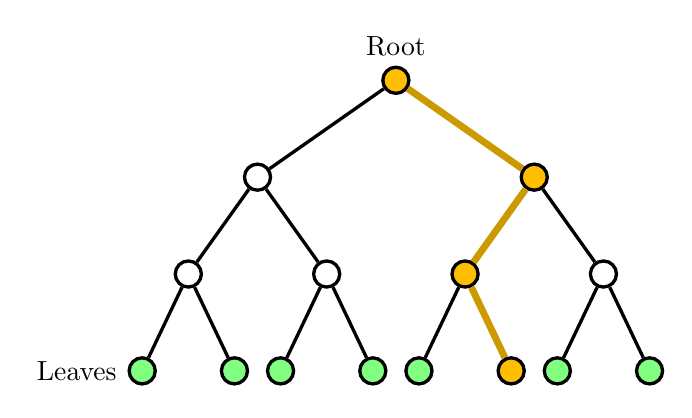
\begin{tikzpicture}[
  level/.style={
    sibling distance = 10.0em/#1,
    level distance = 3.5em
  }
]
\node [node_filled, label={[anchor=south]above:Root}] (root) {}
child [path_normal] {
  node [node] {}
  child {
    node [node] {}
    child {node [node_leaf, label={[anchor=east]left:Leaves}] {}}
    child {node [node_leaf] {}}
  }
  child {
    node [node] {}
    child {node [node_leaf] {}}
    child {node [node_leaf] {}}
  }
}
child [path] {
  node [node_filled] {}
  child {
    node [node_filled] {}
    child [path_normal] {node [node_leaf] {}}
    child {node [node_filled] {}}
  }
  child [path_normal] {
    node [node] {}
    child {node [node_leaf] {}}
    child {node [node_leaf] {}}
  }
};
\end{tikzpicture}
\end{adjustbox}%
          \caption{Binary tree with 15 nodes}%
          \label{fig:binary_tree}%
        \end{centering}%
      \end{figure}
    \end{column}
  \end{columns}
\end{frame}

%-------------------------------------------------------------------------------

\begin{frame}{Runtime - Heapsort 2/6}
  \textbf{Intuitive:}
  \begin{itemize}
    \item
      \textbf{Minsort:}
      To determine the minimum value we have to iterate through all the
      unsorted elements.
    \item
      \textbf{Heapsort:}
      The root-element is always the smallest (min-heap).
      We only need to repair a small part of the full tree after an delete
      operation.
  \end{itemize}
  \textbf{Formal:}
  \begin{itemize}
    \item 
      Let T$(n)$ be the runtime for the \textit{Heapsort}
      algorithm with $n$ elements.
    \item
      On the next pages we will proof $T(n) \leq C \cdot n \, \log_2 n$
  \end{itemize}
\end{frame}